\section{Beta testing}
\begin{center}
\begin{longtable}{|P{30mm}|P{20mm}|P{60mm}|P{25mm}|}
  \hline
  \textbf{Test} & \textbf{Expected result} & \textbf{Actual result} & \textbf{Development guidance} \\
  \hline
  \endfirsthead
  \hline
  \endhead
  \hline 

  \endfoot
  \endlastfoot

Landing page displays login and register buttons & Two buttons are shown
& 
\includegraphics[width=57mm]{ch4_testing_for_eval/media/image1.png}
& No further development needed \\ \hline 
Registration page displays 6 box form for username, password, email and
card details & Form is displayed and the user can enter text &
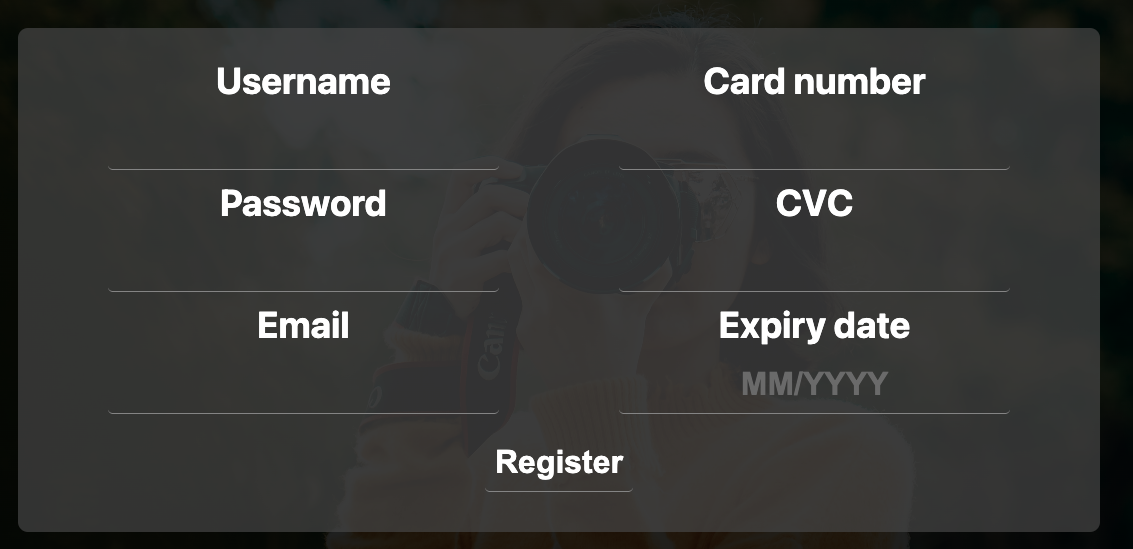
\includegraphics[width=57mm]{ch4_testing_for_eval/media/image2.png} &
Adjust the method of input for the expiry date \\ \hline
User is able to register and then is sent onto the home page & User is
forwarded to the home page &
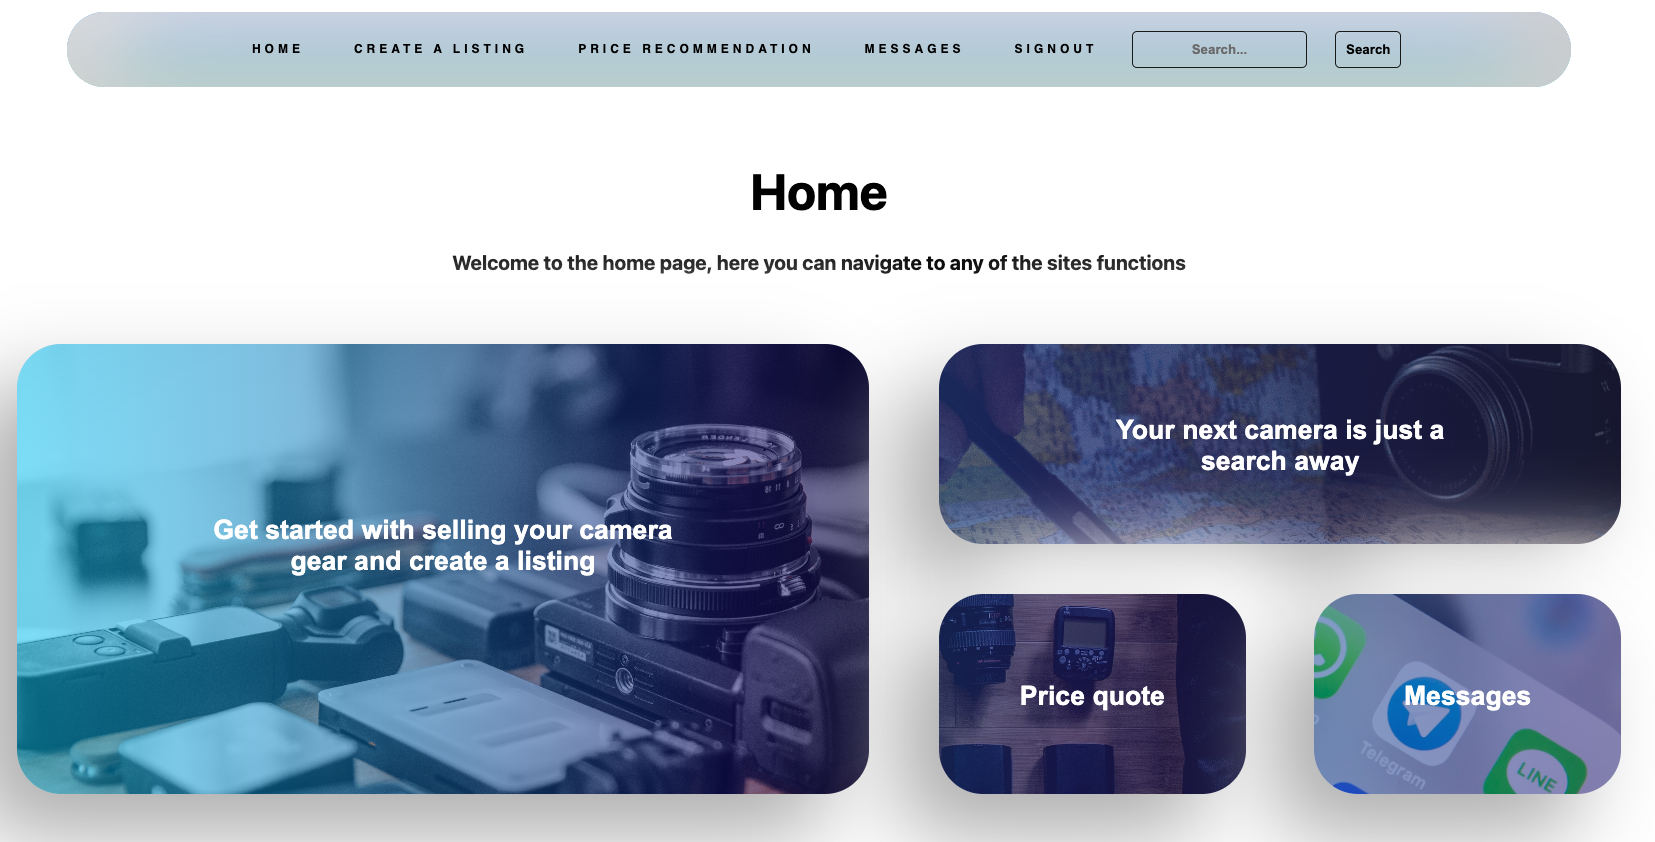
\includegraphics[width=57mm]{ch4_testing_for_eval/media/image6.png} &
Add a specific welcome message for the user \\ \hline
Login page displays username and password box with a forgot password
button & User can see the forgot password button &

\includegraphics[width=57mm]{ch4_testing_for_eval/media/image11.png}
& Move the button so that it sits under the form \\ \hline
If login details are correct the user is forwarded to the home page &
User is sent on to the home page &
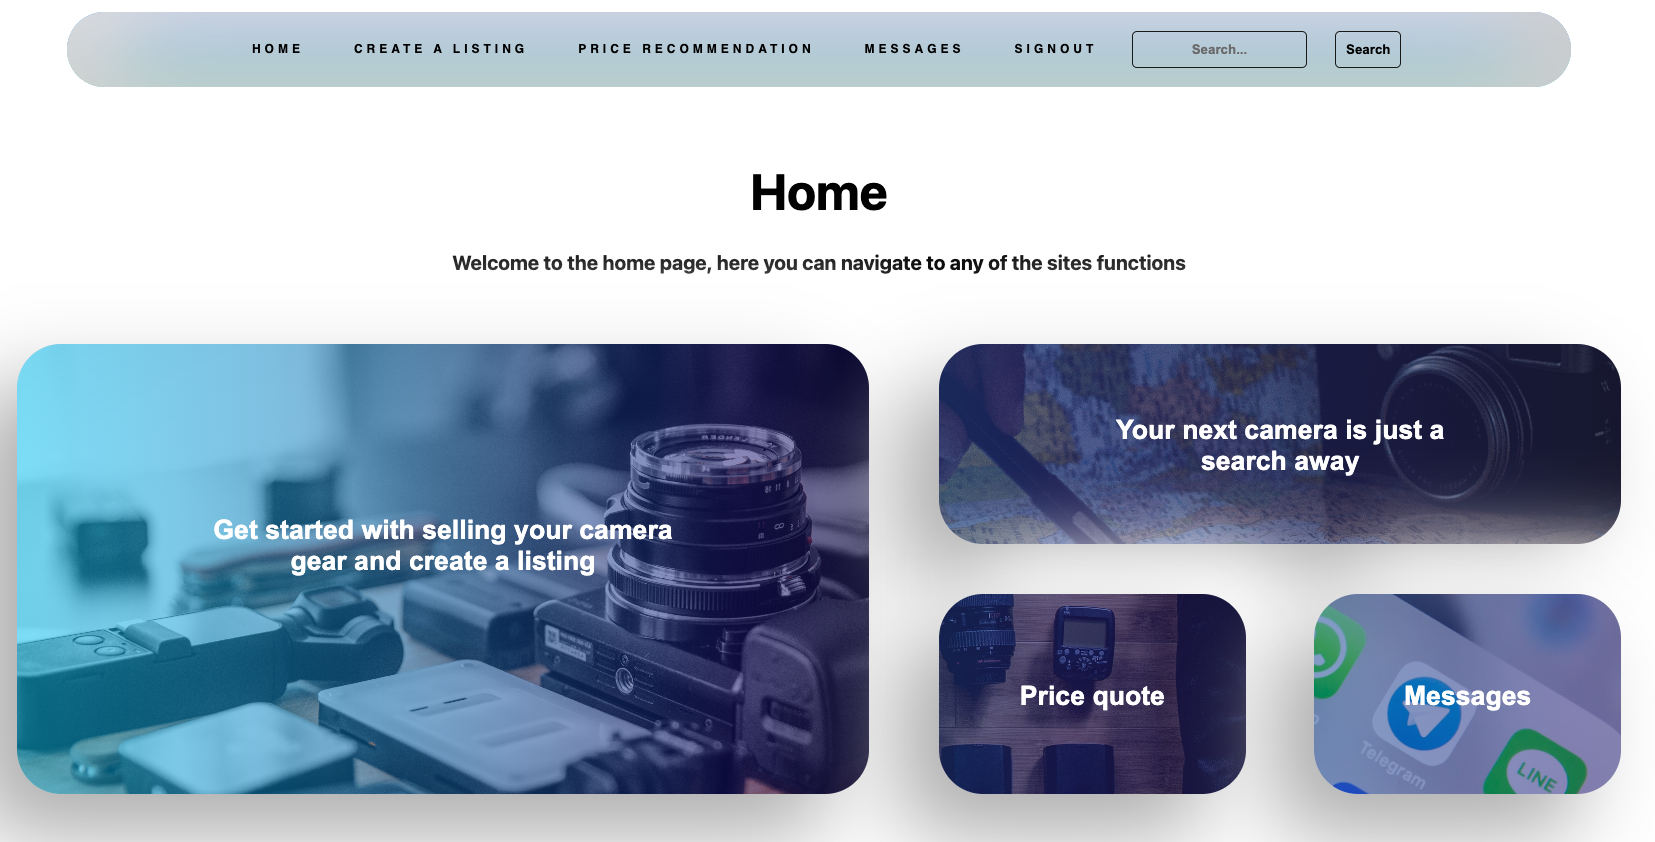
\includegraphics[width=57mm]{ch4_testing_for_eval/media/image6.png} &
Add a specific welcome message for the user \\ \hline
If user forgets password, the form is displayed with username and email
& User is shown another form on the website &
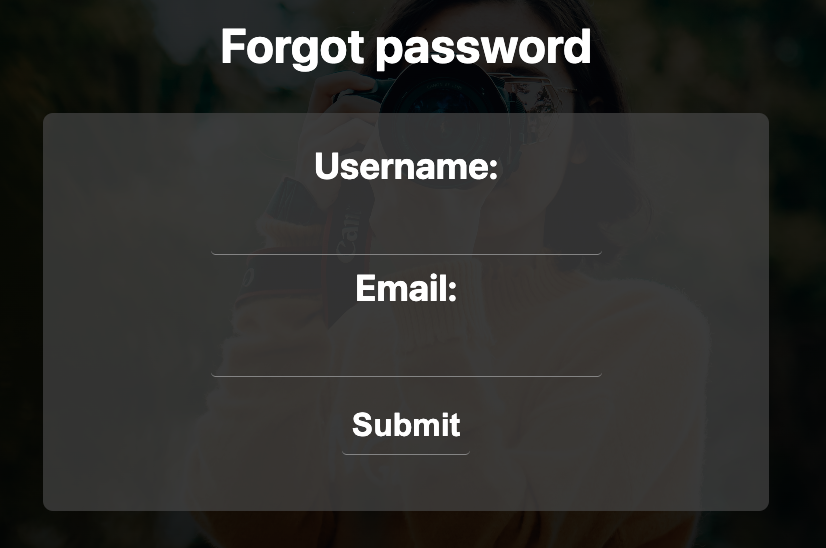
\includegraphics[width=57mm]{ch4_testing_for_eval/media/image12.png}
& No further development \\ \hline
If details are entered correctly, the user is sent a temporary password
by email & User is sent an email with the temporary password &
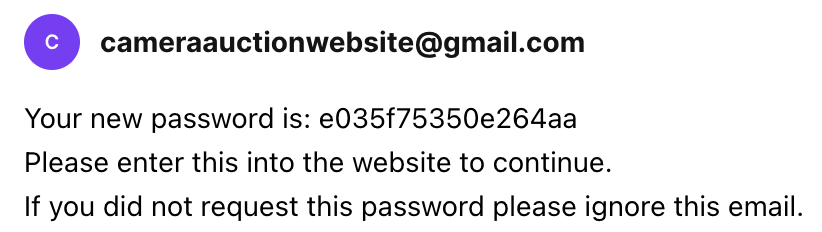
\includegraphics[width=57mm]{ch4_testing_for_eval/media/image47.png}
& Display a better sent message and include the username in the email \\ \hline
Home page is displayed with 4 options of search, create listing, price
quote and messages along with a navigation bar & Home page shows 4
buttons &
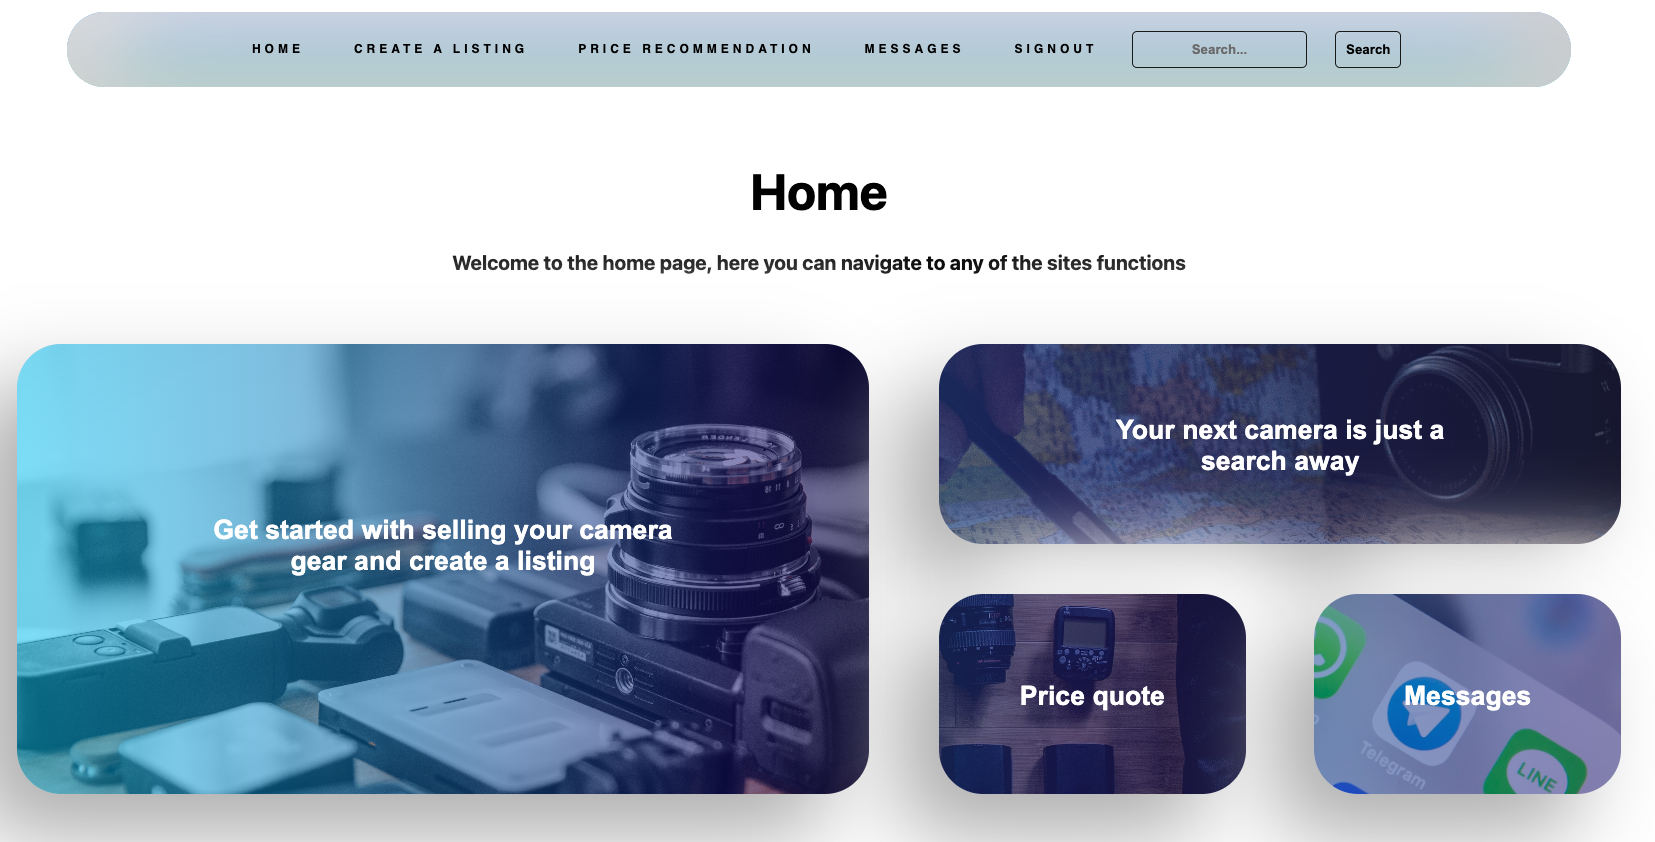
\includegraphics[width=57mm]{ch4_testing_for_eval/media/image6.png} &
No further development \\ \hline
If user selects create a listing, the user is shown a form for all the
camera details & Form is displayed to the user &
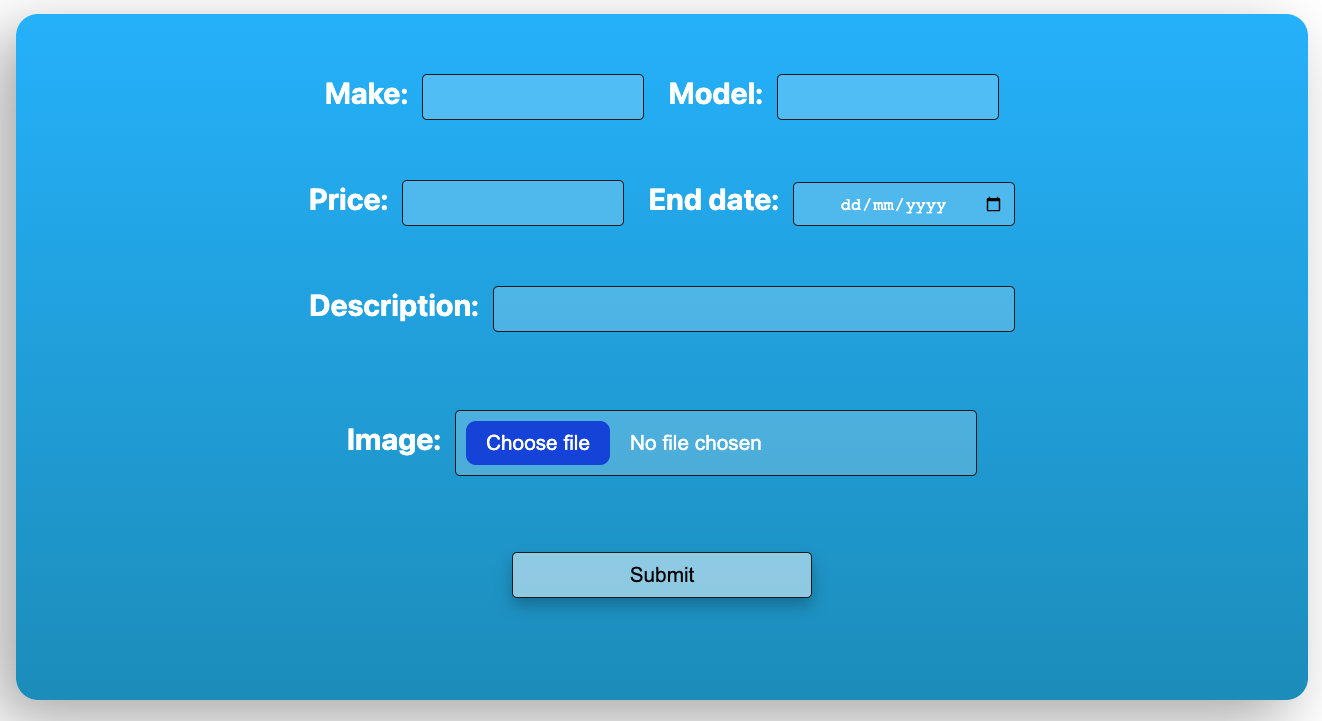
\includegraphics[width=57mm]{ch4_testing_for_eval/media/image20.png}
& Allow the make and model to be selected from a dropdown and increase
the description box size \\ \hline
The user can enter all the cameras details into the form and upload an
image & The form is shown to user and allows the user to upload a file &
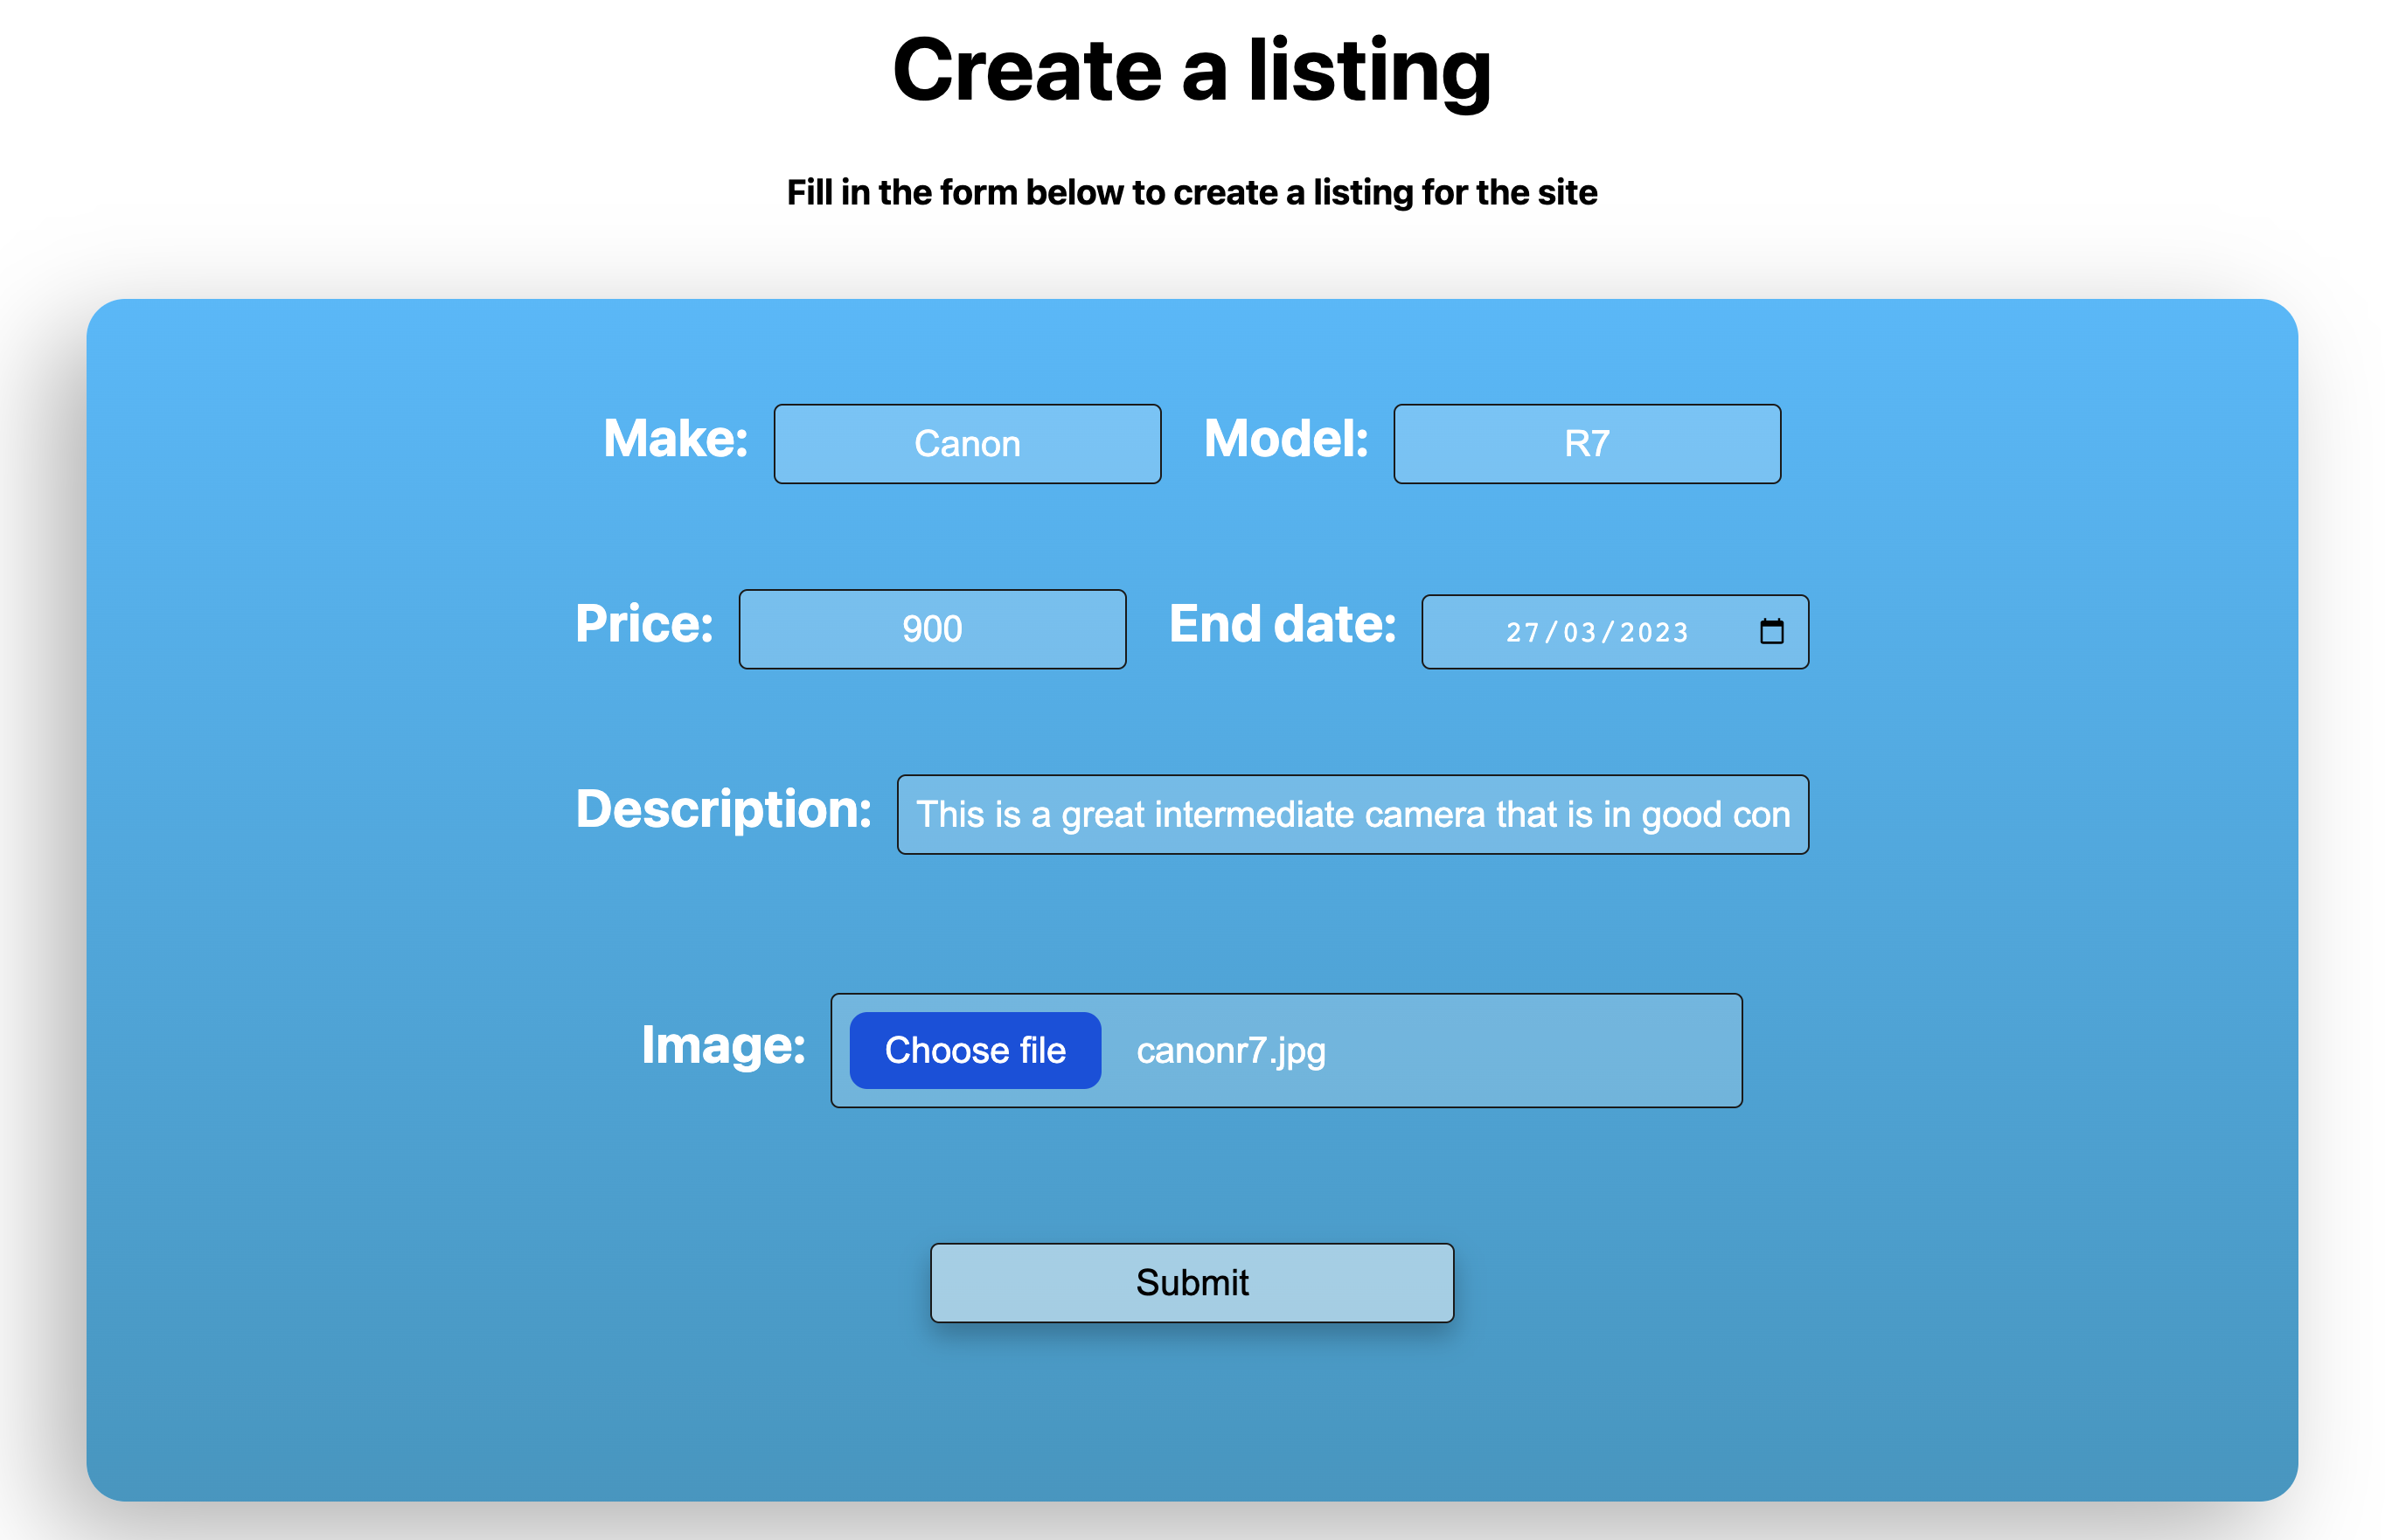
\includegraphics[width=57mm]{ch4_testing_for_eval/media/image48.png}
& Allow the addition of multiple images and increase the description box
size \\ \hline
If all forms are completed correctly then the users listing is uploaded
and sent back to the homepage & Success message then homepage &
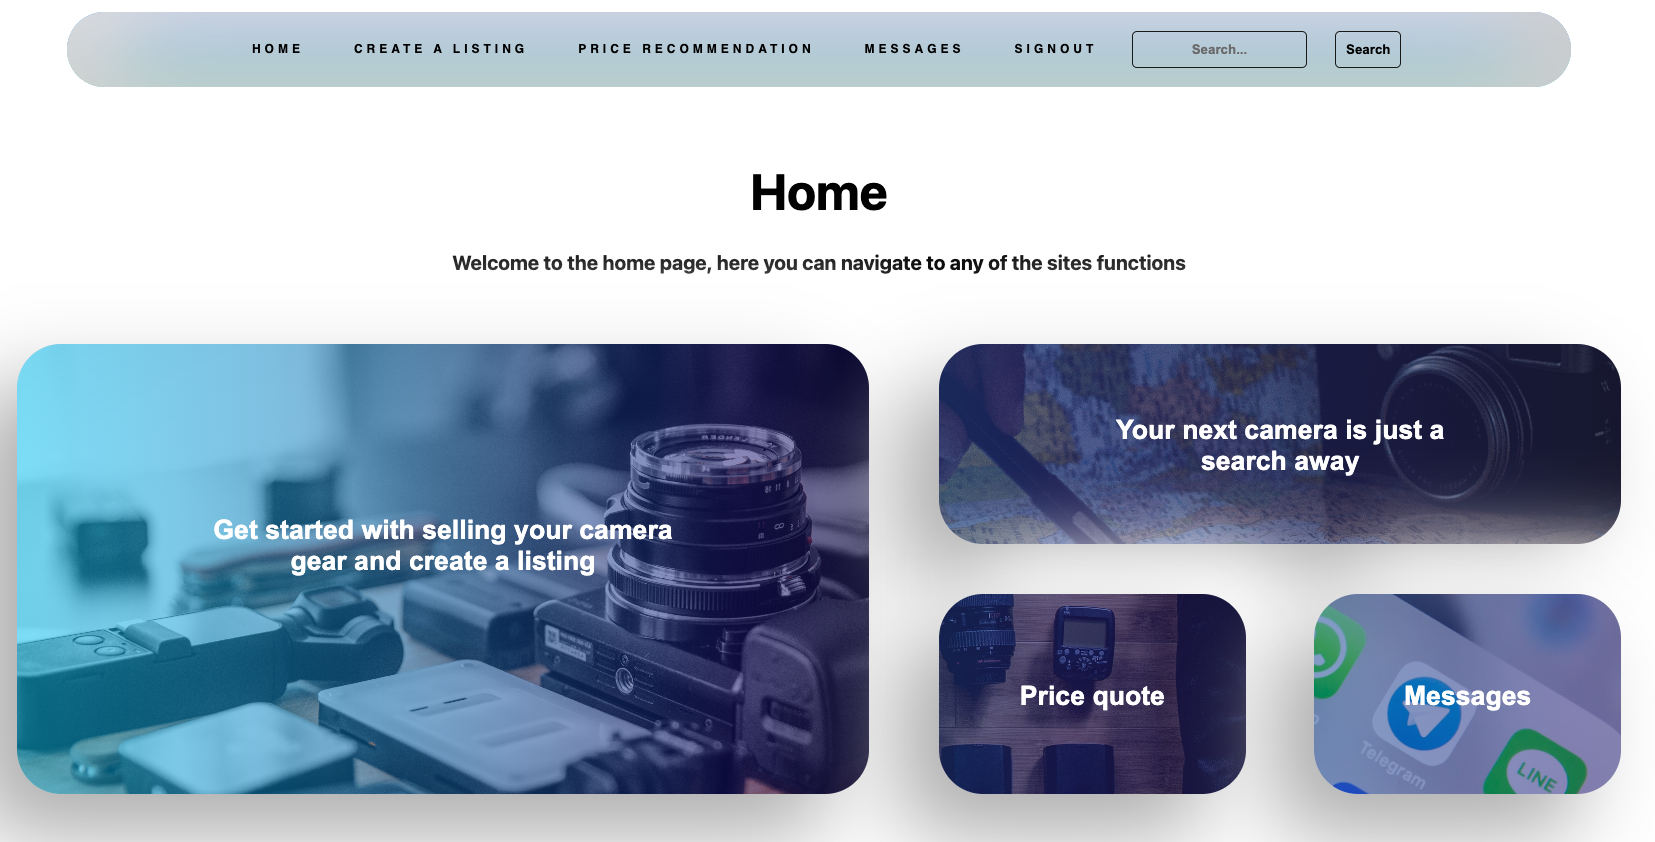
\includegraphics[width=57mm]{ch4_testing_for_eval/media/image6.png} &
Show the user their listing and add a better success message \\ \hline
The user can use the search bar to look for a listing & The user can
enter text and the listings are displayed &

\includegraphics[width=57mm]{ch4_testing_for_eval/media/image27.png}

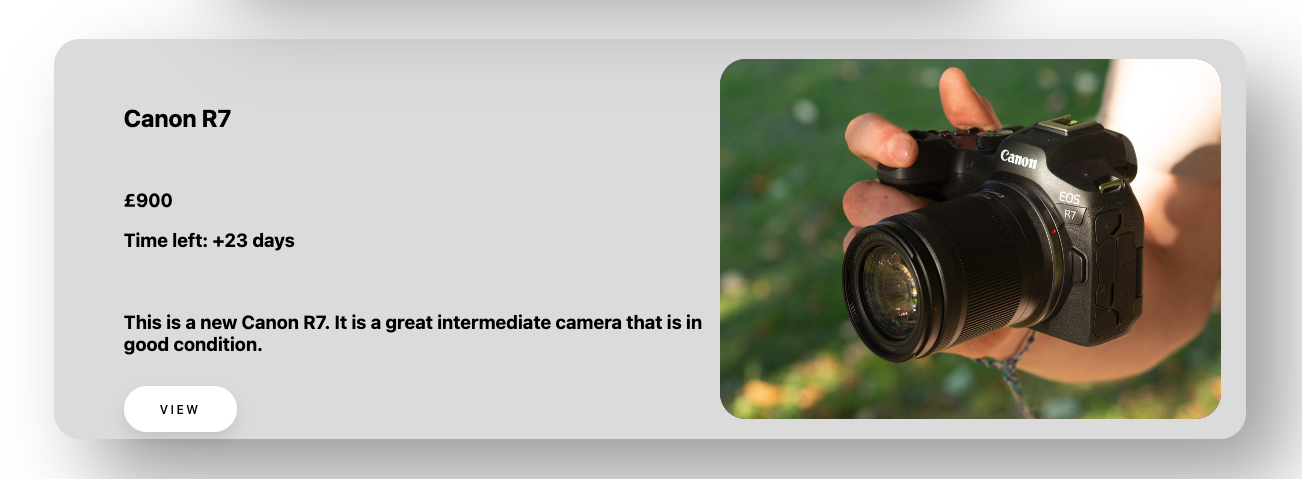
\includegraphics[width=57mm]{ch4_testing_for_eval/media/image28.png}
& No further feedback \\ \hline
All listing results are displayed with all the details and the user can
choose one to follow up or is given an error message if no results are
found & Listings are shown or an error message &
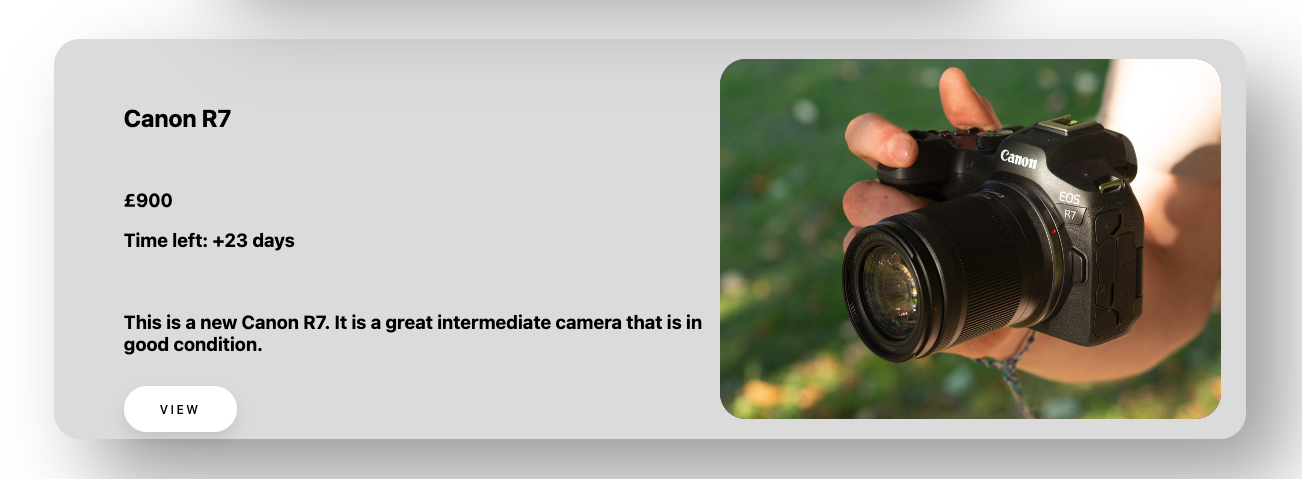
\includegraphics[width=57mm]{ch4_testing_for_eval/media/image28.png}


\includegraphics[width=57mm]{ch4_testing_for_eval/media/image32.png}
& Adjust the formatting of the error message and include a similar items
search \\ \hline
If the user wants to see a full listing, then they are shown the full
listing with an option to bid and message the seller & Full listing is
shown to the user with a bid and message button &
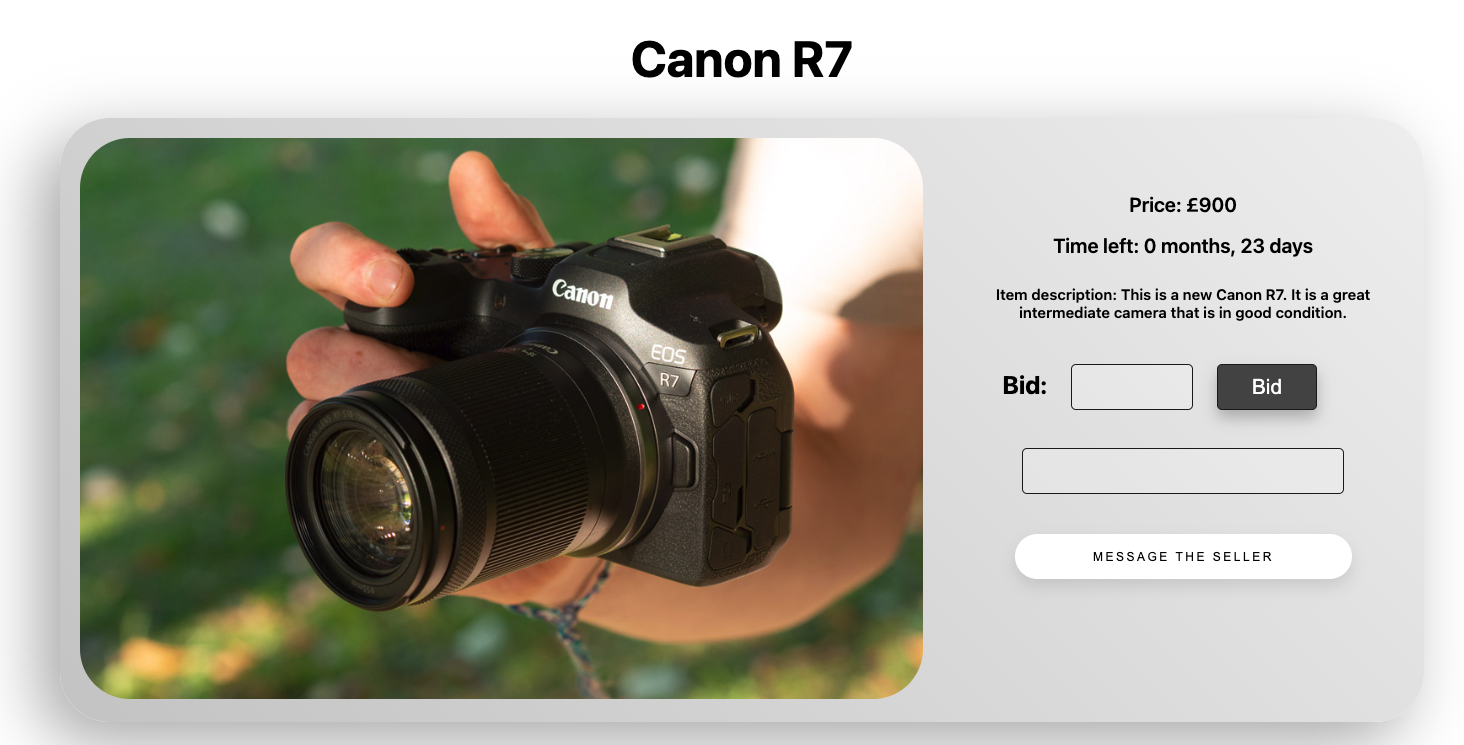
\includegraphics[width=57mm]{ch4_testing_for_eval/media/image33.png}
& All looks correct but add a \\ \hline
The user can enter a bid on an item which is updated and shows the
updated price point & The highest bid is updated &
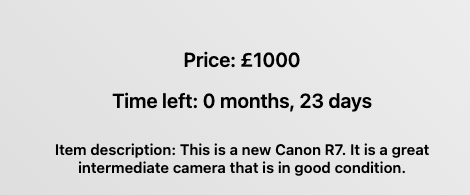
\includegraphics[width=57mm]{ch4_testing_for_eval/media/image34.png}
& Bid updated however would be better is it would show the updated bid
without refresh \\ \hline
The user can enter and submit a message for the seller on the listing &
The user can send the message to the seller &
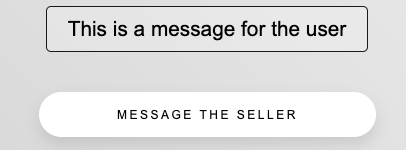
\includegraphics[width=57mm]{ch4_testing_for_eval/media/image37.png}


\includegraphics[width=57mm]{ch4_testing_for_eval/media/image38.png}
& Message is able to be send however it would be good to reply or delete
messages \\ \hline
If the user selects the price recommendation page, they are able to
enter the camera make and model and get a recommendation & User can
enter text and get a price based on sold cameras &
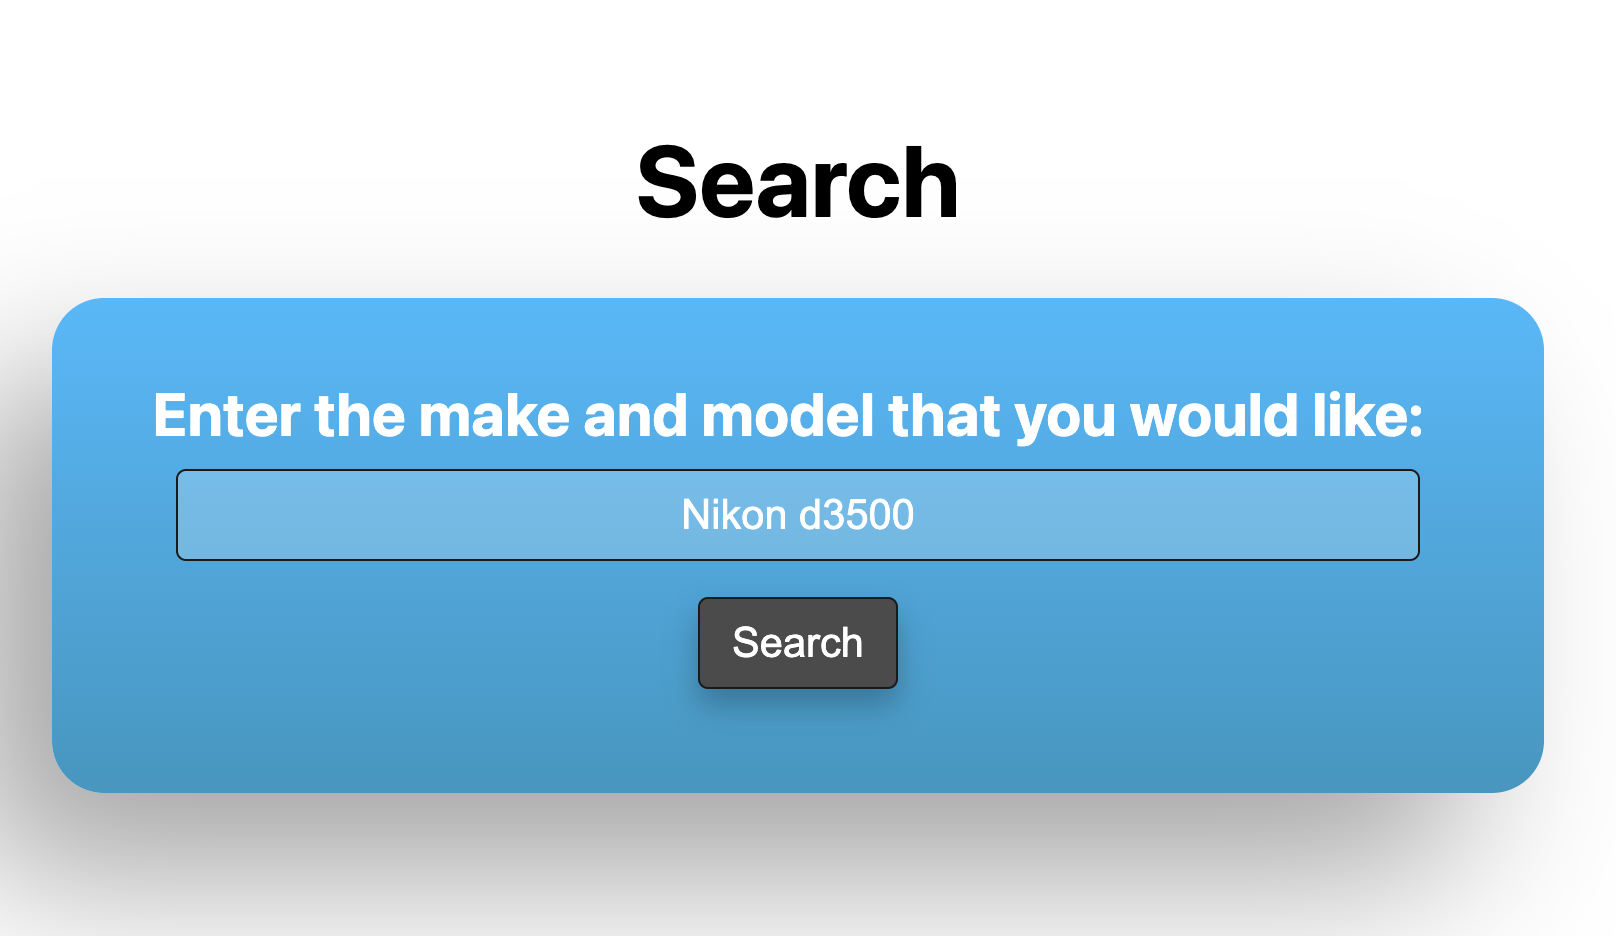
\includegraphics[width=57mm]{ch4_testing_for_eval/media/image49.png}


\includegraphics[width=57mm]{ch4_testing_for_eval/media/image44.png}
& Add a picture of the camera and perhaps sold cameras of the same brand
as well \\ \hline
If the user selects messages, then they are able to see all the messages
that have been sent to them and who they are from & Messages are shown
to the user &

\includegraphics[width=57mm]{ch4_testing_for_eval/media/image38.png}
& Add a way to reply to and delete the messages that have been sent \\ \hline

    \caption{Beta testing table}
\label{tab:beta_testing}
\end{longtable}
\end{center}